\documentclass{beamer}

\usepackage[T1]{fontenc}       
\usepackage[utf8]{inputenc}    % pour les accents (mettre latin1 pour windows au lieu de utf8)
\usepackage[frenchb]{babel}    % le documents est en français

\usepackage{xcolor}            % pour définir plus de couleurs 
\usepackage{graphicx}          % pour insérer des figures

\usepackage{animate}

\usepackage{amsmath,amsfonts,amssymb,dsfont}
\usepackage{amsthm,stmaryrd}

\usepackage{graphicx}
\usepackage{caption}
\captionsetup{compatibility=false}
\usepackage{subcaption}
\usepackage[justification=centering]{caption}
%\usepackage{floatrow}

\usetheme{Darmstadt}

\setbeamertemplate{navigation symbols}{
}

\usepackage{remreset}
\makeatletter
\@removefromreset{subsection}{section}
\makeatother
\setcounter{subsection}{1}

\title[]{Overcoming Partial Observability with RNNs}
\author{Guillaume Berger}
\date{\today}


\begin{document}

\begin{frame}
	\titlepage
%	\begin{figure}[!h]
%	\centering
%	\includegraphics[width=0.2\textwidth]{C:/Users/Guillaume/Desktop/ECLille/G3/Master/Memoire/Presentation/CentraleLogo.png}
%	\end{figure}
\end{frame}

\begin{frame}{The limit of DQNs and POMDPs}
	
	\textbf{Partial Observability:}
	
	\begin{itemize}
		\item in most real-world applications, the entire world is not visible at any moment, but partially observable
		\item MDP $\Rightarrow$ \textbf{POMDP}
	\end{itemize}
	
	\vspace{0.5cm}
	
	\textbf{The limit of DQNs:} the input receptive field is fixed
	
	\begin{figure}[!h]
		\centering
		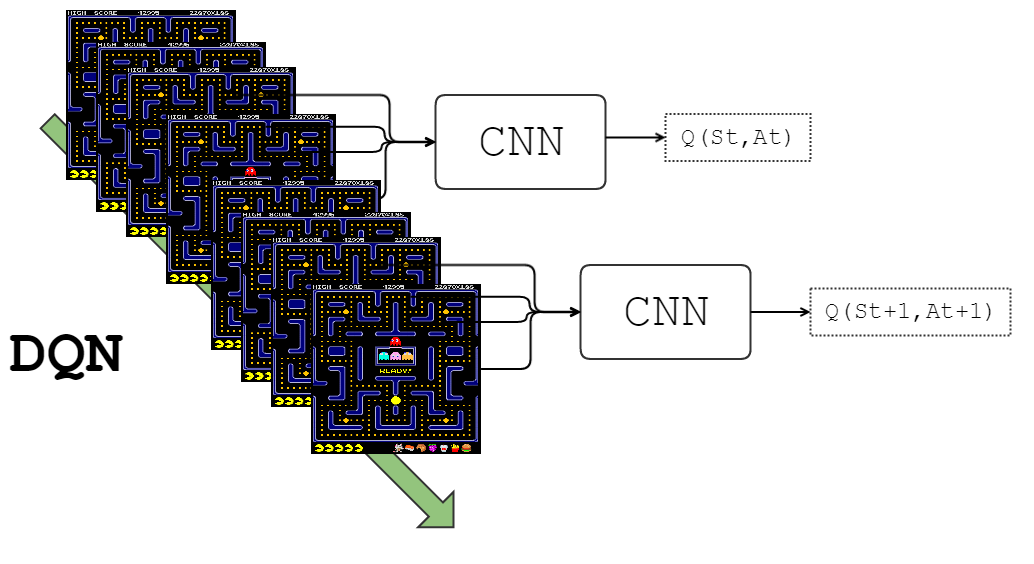
\includegraphics[width=0.8\textwidth]{imgs/DQN.png}
	\end{figure}
	
\end{frame}

\begin{frame}{RNNs and Memory Networks}
	
	Recurrency might help:
	$h_{t+1} = \Phi(U \ x_{t+1}  +  W \ h_t) $
	
	Implement and compare \textbf{different neural architectures} on \textbf{POMDPs} trained via \textbf{deep Q-learning}
	
	\begin{figure}[!h]
		\centering
		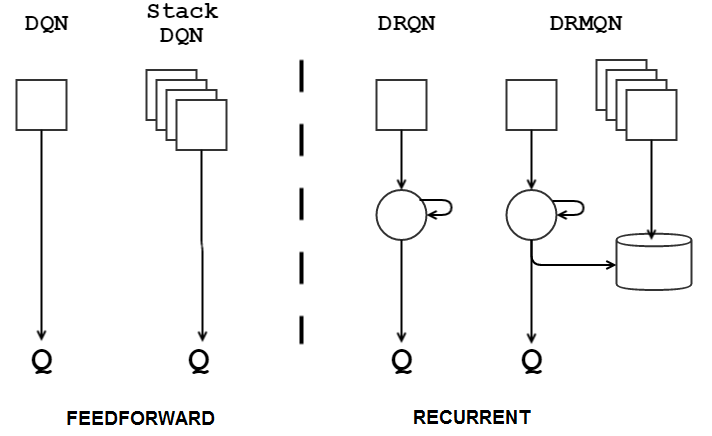
\includegraphics[width=0.9\textwidth]{imgs/schema_archi.png}
	\end{figure}

\end{frame}

\begin{frame}{Environments}
	
	\textbf{Experiment A : the myopic agent}
	
	\begin{figure}
			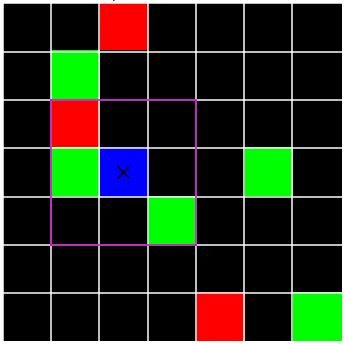
\includegraphics[height=6cm]{imgs/myopic.png}
	\end{figure}	

\end{frame}

\begin{frame}{Learning curves}
	\begin{figure}
		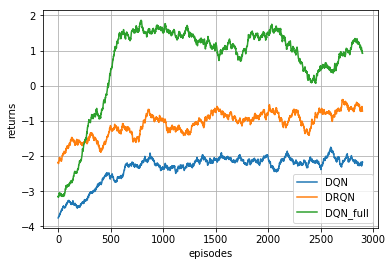
\includegraphics[height=7.5cm]{imgs/myopic_curves.png}
	\end{figure}
\end{frame}

\begin{frame}{Environments}
	
	\textbf{Experiment B : the masked agent}
	
	\begin{figure}
			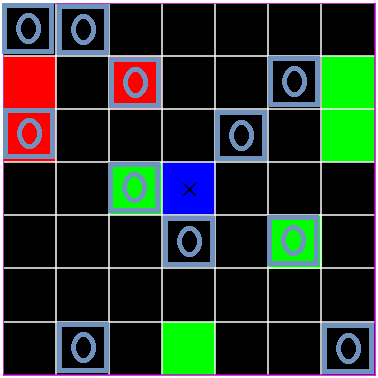
\includegraphics[height=6cm]{imgs/masked.png}
	\end{figure}
	
	Dropout rate : $P$
\end{frame}

\begin{frame}{Learning curves}
	\begin{figure}
		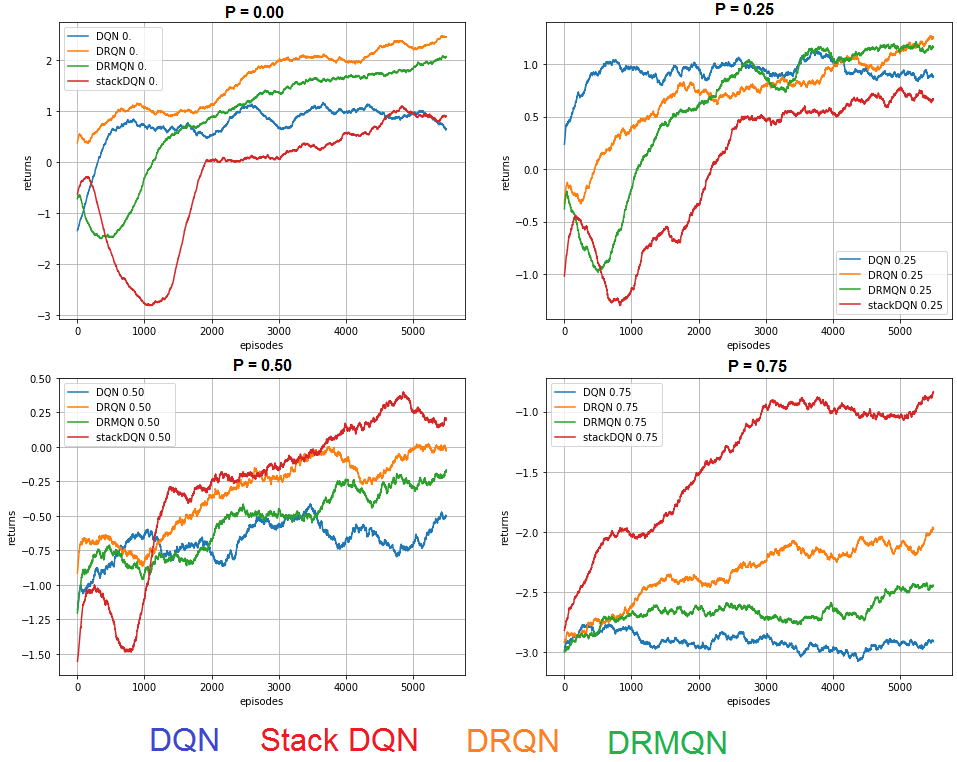
\includegraphics[height=7cm]{imgs/masked_curves.png}
	\end{figure}
\end{frame}



\begin{frame}{Robustness to partial observability}
	
	\begin{itemize}
		\item Training in a fully observable scenario (i.e. no mask, $P=0$), but \textbf{testing with partial observability ($P=0.5$)}.
		\item Experiment held on the ``Masked'' case.
	\end{itemize}
	
	\begin{table}[]
		\centering
		\caption{Average return for each architecture}
		\label{my-label}
		\begin{tabular}{|c|c|c|c|}
			\hline
			DQN & Stack DQN & DRQN        & DRMQN       \\ \hline
			-2.05  & -1.27  & -1.31 & -1.45 \\ \hline
		\end{tabular}
	\end{table}
	
\end{frame}

\begin{frame}{References}
	
	[1] Deep Recurrent Q-Learning for Partially Observable MDPs, Matthew Hausknecht and Peter Stone, (2015) \vspace{0.3cm}
	
	[2] Playing Atari with Deep Reinforcement Learning, Volodymyr Mnih, Koray Kavukcuoglu, David Silver, Alex Graves, Ioannis Antonoglou, Daan Wierstra, Martin Riedmiller (2015) \vspace{0.3cm}
	
	[3] Control of Memory, Active Perception, and Action in Minecraft, Junhyuk Oh, Valliappa Chockalingam, Satinder Singh, Honglak Lee (2016)
	
\end{frame}


\begin{frame}{Diferentiable memory module}
	
	[4] End-To-End Memory Networks, Sainbayar Sukhbaatar, Arthur Szlam, Jason Weston, Rob Fergus (2015)
	
	\begin{figure}
		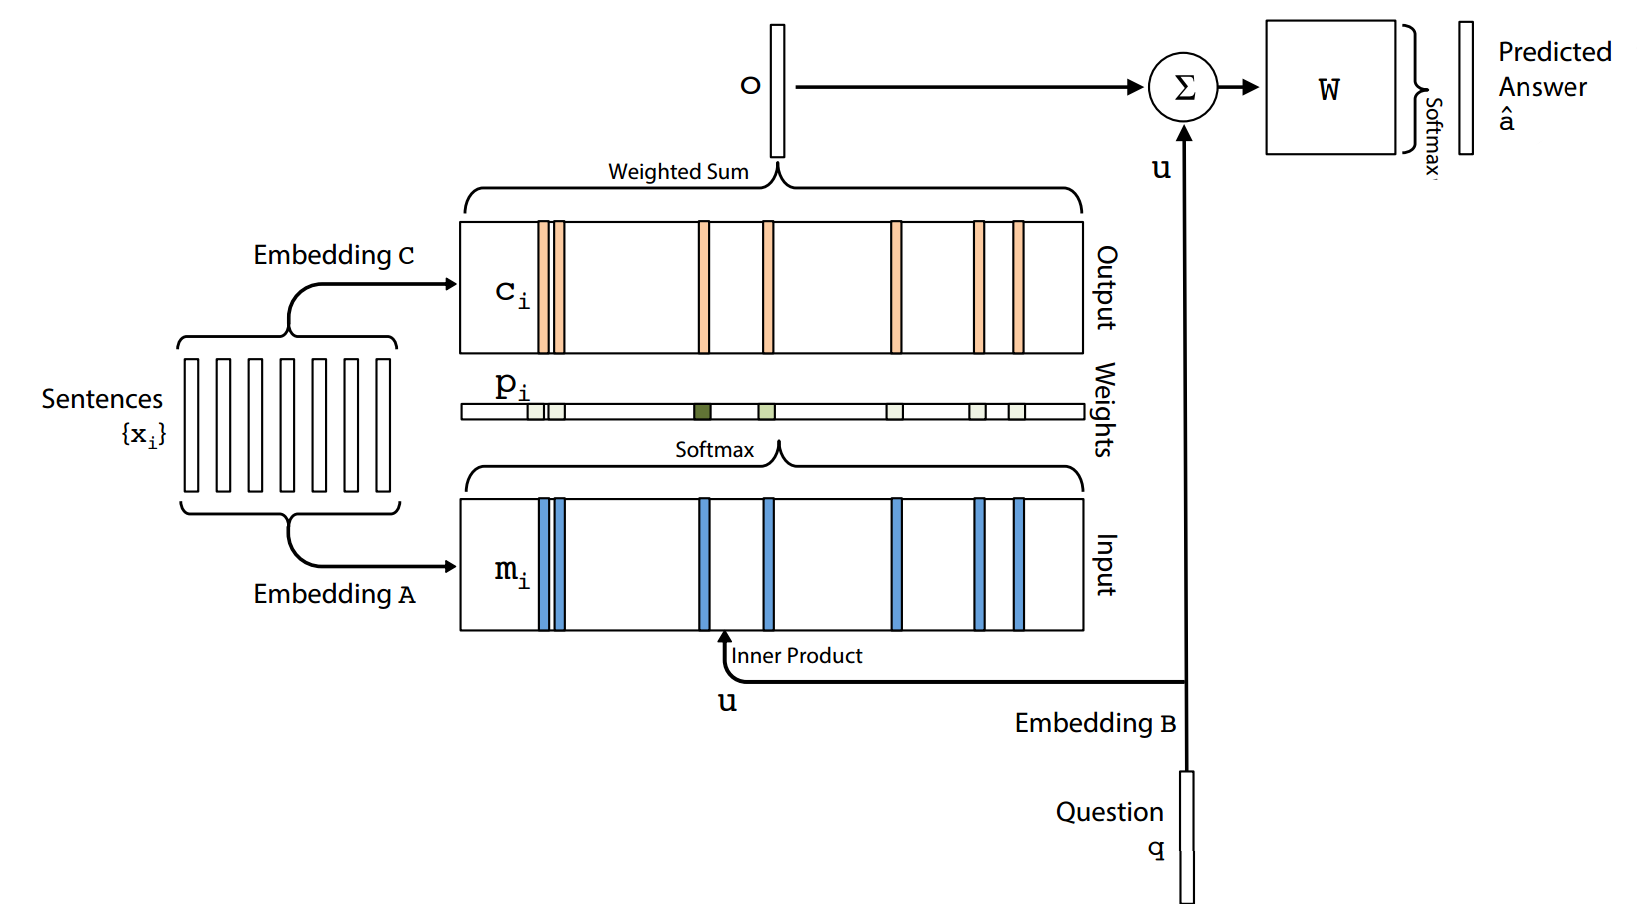
\includegraphics[height=6cm]{imgs/memory_module.png}
	\end{figure}
	
\end{frame}

\end{document}
